\section{Auswertung}

\subsection{Durchlasskennlinie Polarisator/Analysator-Paar}

Die  Durchlasskennlinie  des Polarisator/Analysator-Paars  wurde  gemessen.  Die
erste   Messung  ist  in  der  Abbildung  \ref{fig:aufgabe-3_falsch}  zu  sehen.

\begin{figure}[H]
    \centering
    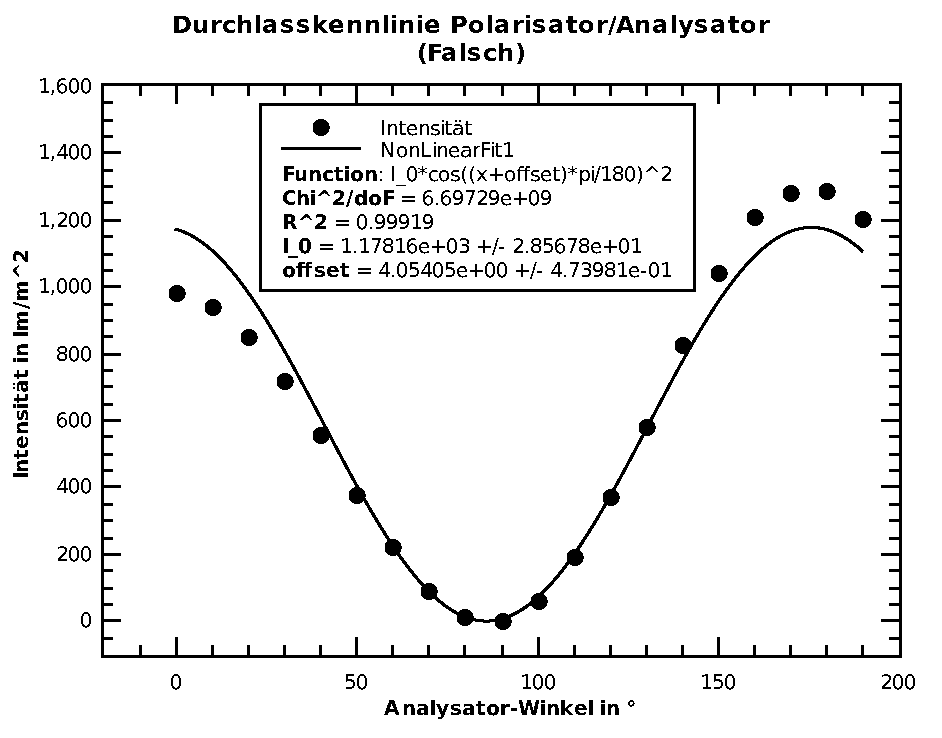
\includegraphics[width=.6\linewidth]{images/aufgabe-3_falsch.pdf}
    \caption{Die erste (inkorrekte) Messung der Durchlasskennlinie}
    \label{fig:aufgabe-3_falsch}
\end{figure}

Es  wurde  bemerkt,  dass  die  Spitzenwerte  bei  jeweils  \SI{0}{\degree}  und
\SI{180}{\degree} nicht gleich sind. Weiter wurde bemerkt,  dass  die  einzelnen
Punkte nach der \SI{90}{\degree}-Einstellung nicht korrekt ``gespiegelt'' werden
konnten.

Die  Messeinrichtung   wurde   nochmals  \"uberpr\"uft,  die  Ausrichtungen  der
Polarisatoren  wurde  justiert,  und die Messung wurde nochmals  durchgef\"uhrt.
Abbildung \ref{fig:aufgabe-3} zeigt die zweite Messung.

\begin{figure}[H]
    \centering
    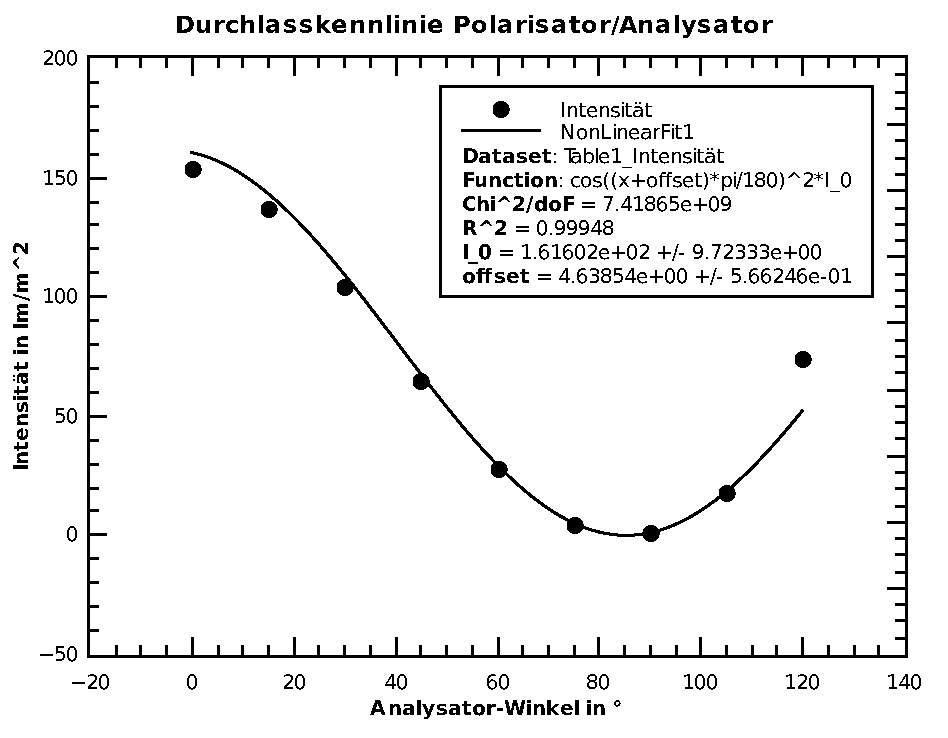
\includegraphics[width=.6\linewidth]{images/aufgabe-3.pdf}
    \caption{}
    \label{fig:aufgabe-3}
\end{figure}

Die  gemessene  Abweichung  scheint  immer  noch  vorhanden  zu  sein.  Es liegt
warscheinlich daran, dass der Analysator nicht ganz zentriert ist und deshalb in
der gegenrotierten Richtung eine andere Durchlasskennlinie hat.

Die Punkte wurden mit der  Formel  \ref{eq:pol_paar}  gefittet,  aber  mit einer
kleinen Anpassung. Die Polarisatoren sind in der Messeinrichtung nicht ganz  bei
\SI{0}{\degree}, es besteht ein unbekannter Offset. Die Formel wurde angepasst:

\begin{equation}
    I_{out} = I_0\cdot\cos^2(\varphi + \varphi_{offset})
\end{equation}

Aus den Fits ist zu lesen:

\begin{align*}
    I_{0,1}            &= 1178.2 \pm 28.568\SI{}{\lumen\per\square\meter} \\
    I_{0,2}            &= 161.60 \pm 9.6233\SI{}{\lumen\per\square\meter} \\
    \varphi_{offset,1} &= 4.0540 \pm 0.4740\SI{}{\degree} \\
    \varphi_{offset,2} &= 4.6385 \pm 0.5663\SI{}{\degree} \\
\end{align*}

Dabei ist zu beachten: $I_{0,1}$ weicht zu stark  ab  weil  die  Messeinrichtung
verstellt  wurde.   Der  Offset  $\varphi_{offset,1}$  kann  jedoch  immer  noch
verwendet   werden,   weil   der   Polarisatorwinkel   nicht  verstellt   wurde.


\subsection{Drehung einer Halbwellenplatte}

Eine Halbwellenplatte wurde zwischen Polarisator und  Analysator  platziert. Bei
verschiedenen Winkeln  wurde  der  Ausl\"oschwinkel  des  Analysators  gemessen.

\begin{figure}[H]
    \centering
    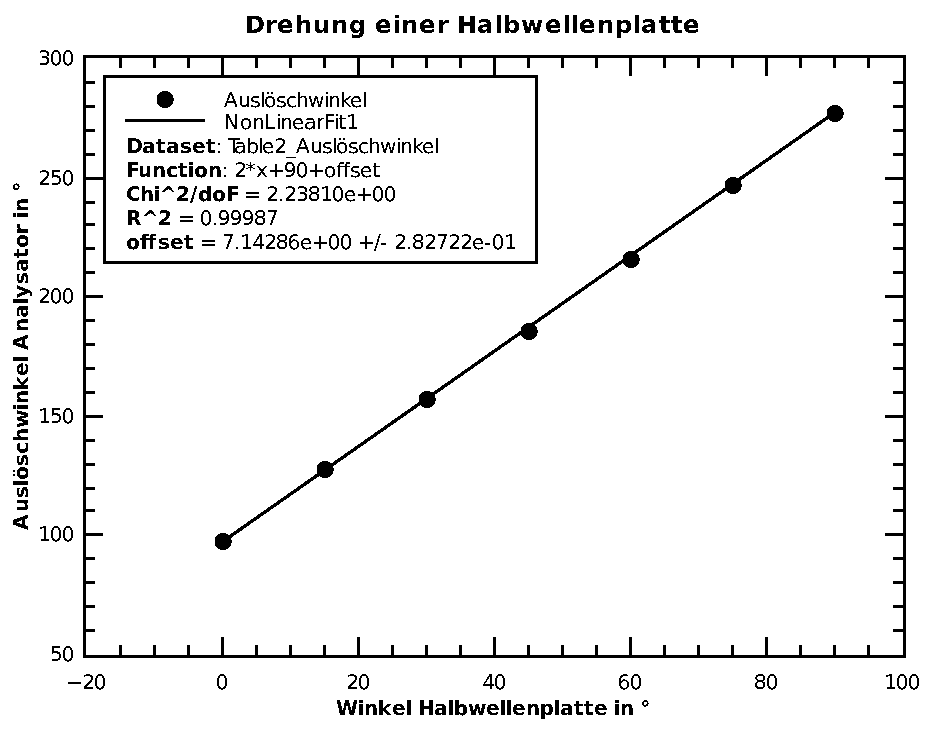
\includegraphics[width=.6\linewidth]{images/aufgabe-4.pdf}
    \caption{}
\end{figure}

Gem\"ass Theorie muss eine Winkel\"anderung der  Halbwellenplatte $\varphi$ eine
verdoppelte Rotation des Ausl\"oschwinkels verursachen.

Wieder muss der unbekannte Offset miteinbezogen werden. Die Fit-Funktion lautet:

\begin{equation}
    \vartheta = 2\varphi + 90 + \varphi_{offset}
\end{equation}

Die  \SI{90}{\degree}  sind dort weil der Ausl\"oschwinkel bei  \SI{90}{\degree}
sein sollte.

Aus dem Fit ist zu lesen:

\begin{align*}
    \varphi_{offset,3} = 7.1429 \pm 0.2827\SI{}{\degree}
\end{align*}


\subsection{Durchlasskennlinie einer Viertelwellenplatte}

Eine Viertelwellenplatte wurde  zwischen  Polarisator  und Analysator platziert.
Bei    verschiedenen    Winkeleinstellungen   $\varphi$    =    \SI{0}{\degree},
\SI{15}{\degree},  \SI{30}{\degree},  \SI{45}{\degree},   \SI{60}{\degree}   der
Platte   wurde   die   Durchlasskennlinie  $I(\varphi,   \vartheta)$   gemessen.

\begin{figure}[H]
    \centering
    \begin{subfigure}{.45\linewidth}
        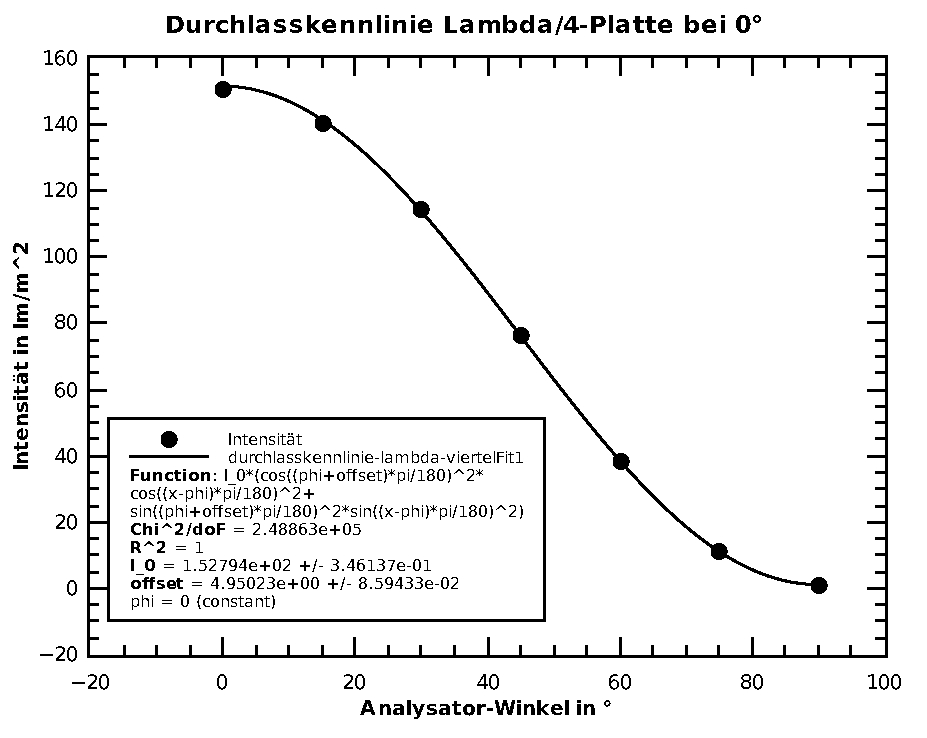
\includegraphics[width=\linewidth]{images/aufgabe-5_0grad.pdf}
    \end{subfigure}
    \begin{subfigure}{.45\linewidth}
        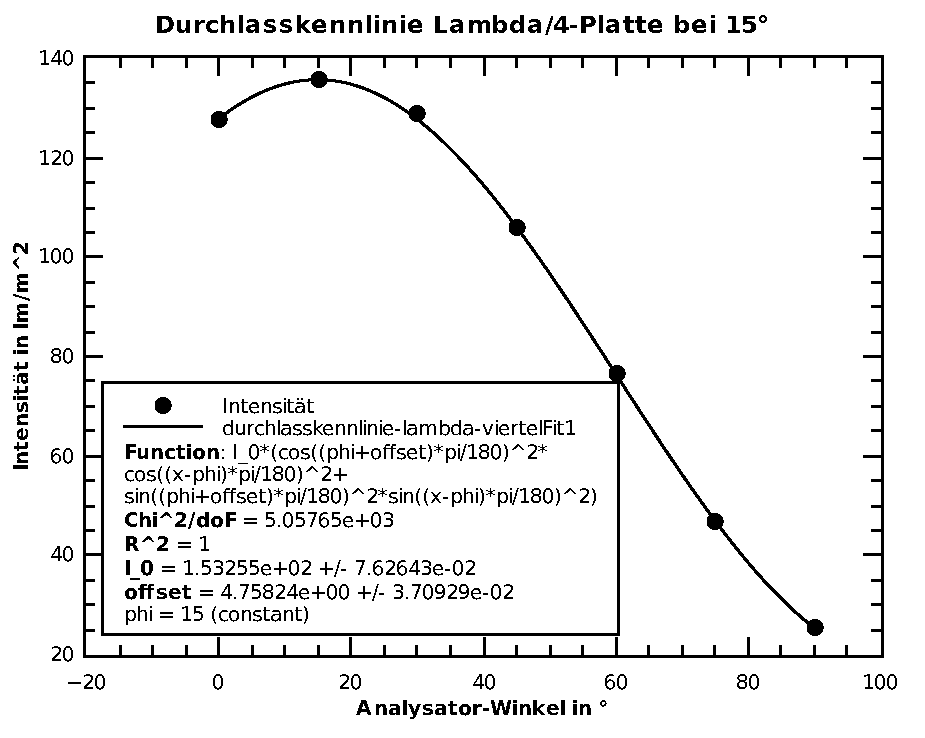
\includegraphics[width=\linewidth]{images/aufgabe-5_15grad.pdf}
    \end{subfigure}
    \begin{subfigure}{.45\linewidth}
        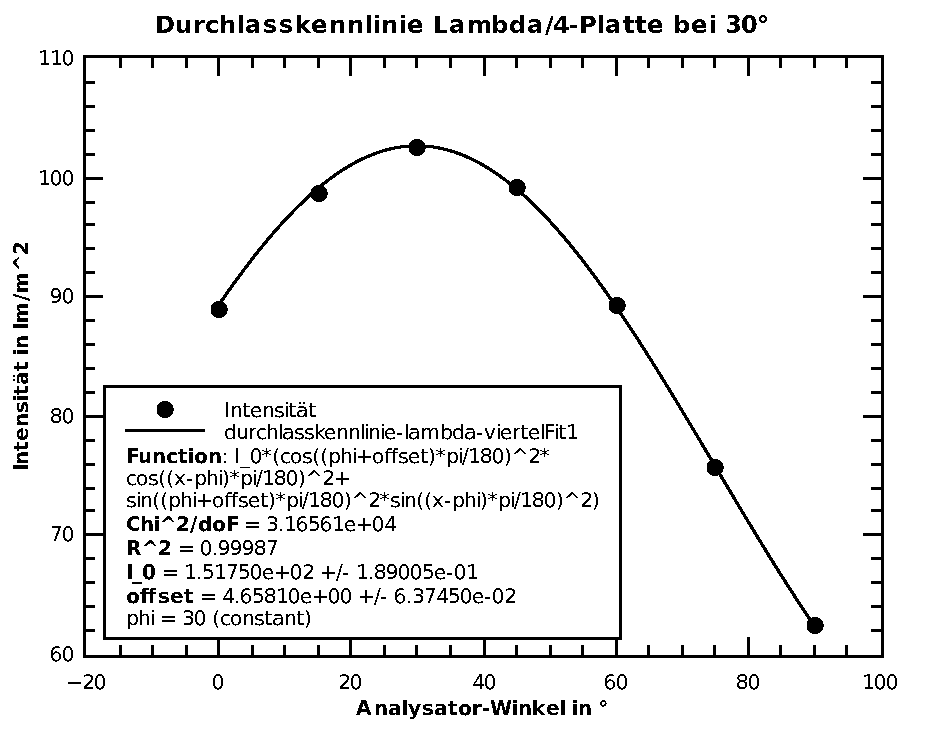
\includegraphics[width=\linewidth]{images/aufgabe-5_30grad.pdf}
    \end{subfigure}
    \begin{subfigure}{.45\linewidth}
        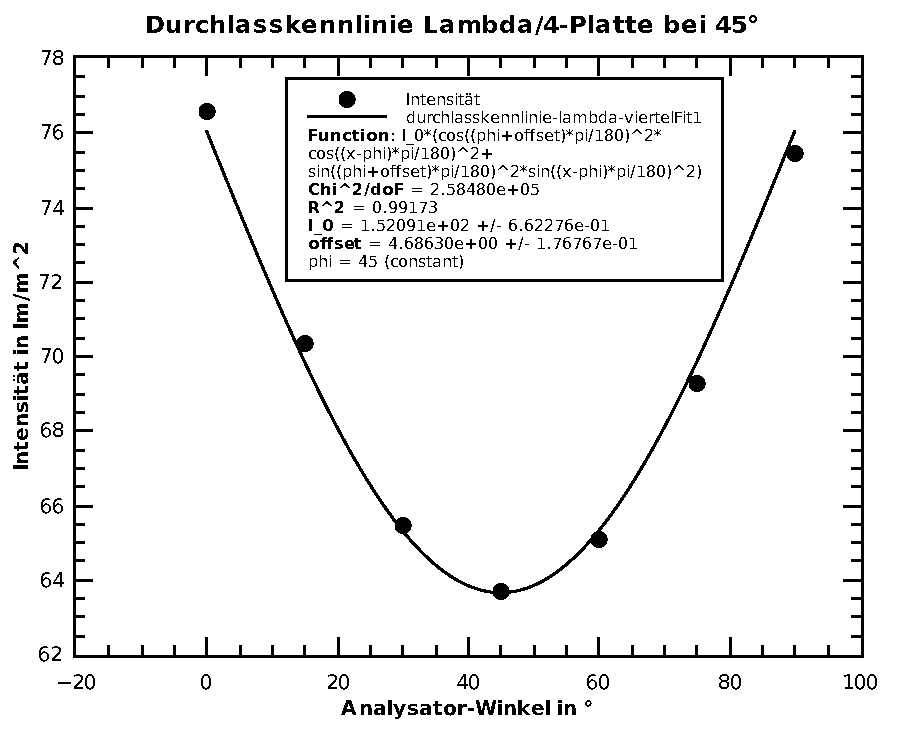
\includegraphics[width=\linewidth]{images/aufgabe-5_45grad.pdf}
    \end{subfigure}
    \begin{subfigure}{.45\linewidth}
        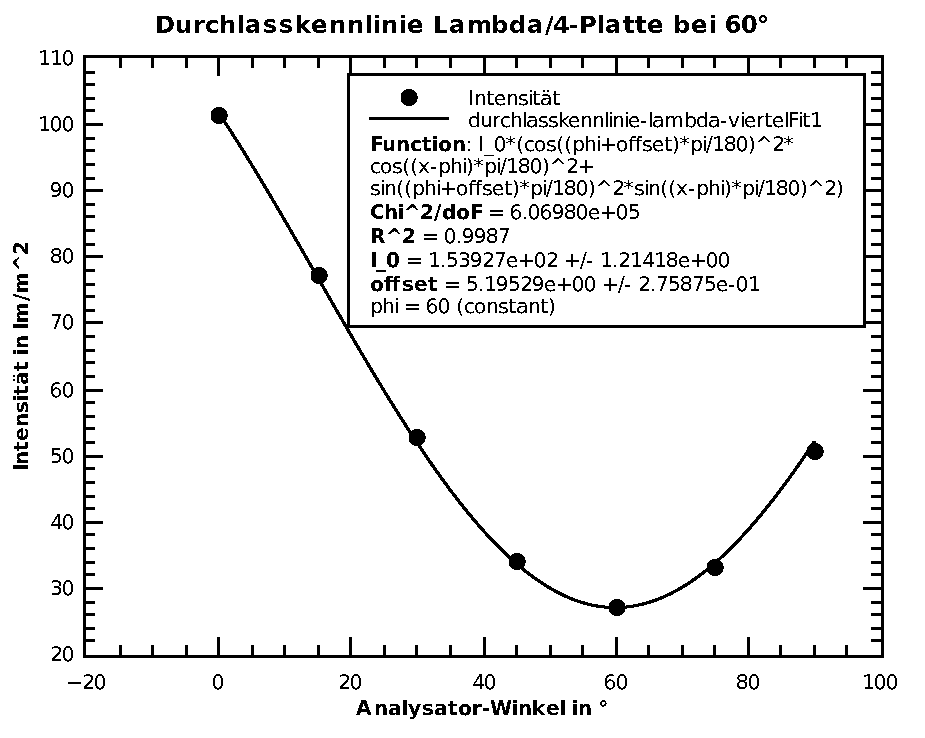
\includegraphics[width=\linewidth]{images/aufgabe-5_60grad.pdf}
    \end{subfigure}
    \caption{}
\end{figure}
Gem\"ass Theorie  kann die Formel der Viertelwellenplatte angewendet werden. Die
Formel \ref{eq:intensitaet} wurde angepasst, damit der unbekannte Offset  wieder
gefittet werden kann:

\begin{equation}
    I = I_0\left(\cos^2(\varphi+\varphi_{offset})\cos^2(\vartheta-\varphi) + \sin^2(\varphi+\varphi_{offset})\sin^2(\vartheta-\varphi)\right)
\end{equation}

Aus dem Fit kann gelesen werden:

\begin{align*}
    I_{0,4} &= 152.794 \pm 0.3461\SI{}{\lumen\per\square\meter} & \varphi_{offset,4} &= 4.9502 \pm 0.0859\SI{}{\degree} \\
    I_{0,5} &= 153.255 \pm 0.0763\SI{}{\lumen\per\square\meter} & \varphi_{offset,5} &= 4.7582 \pm 0.0370\SI{}{\degree} \\
    I_{0,6} &= 151.750 \pm 0.1890\SI{}{\lumen\per\square\meter} & \varphi_{offset,6} &= 4.6581 \pm 0.0637\SI{}{\degree} \\
    I_{0,7} &= 152.091 \pm 0.0662\SI{}{\lumen\per\square\meter} & \varphi_{offset,7} &= 4.6863 \pm 0.1768\SI{}{\degree} \\
    I_{0,8} &= 153.927 \pm 1.2142\SI{}{\lumen\per\square\meter} & \varphi_{offset,8} &= 5.1953 \pm 0.2759\SI{}{\degree} \\
\end{align*}


\subsection{Durchlasskennlinie mit Gr\"unes Laserlicht}

\begin{figure}[H]
    \centering
    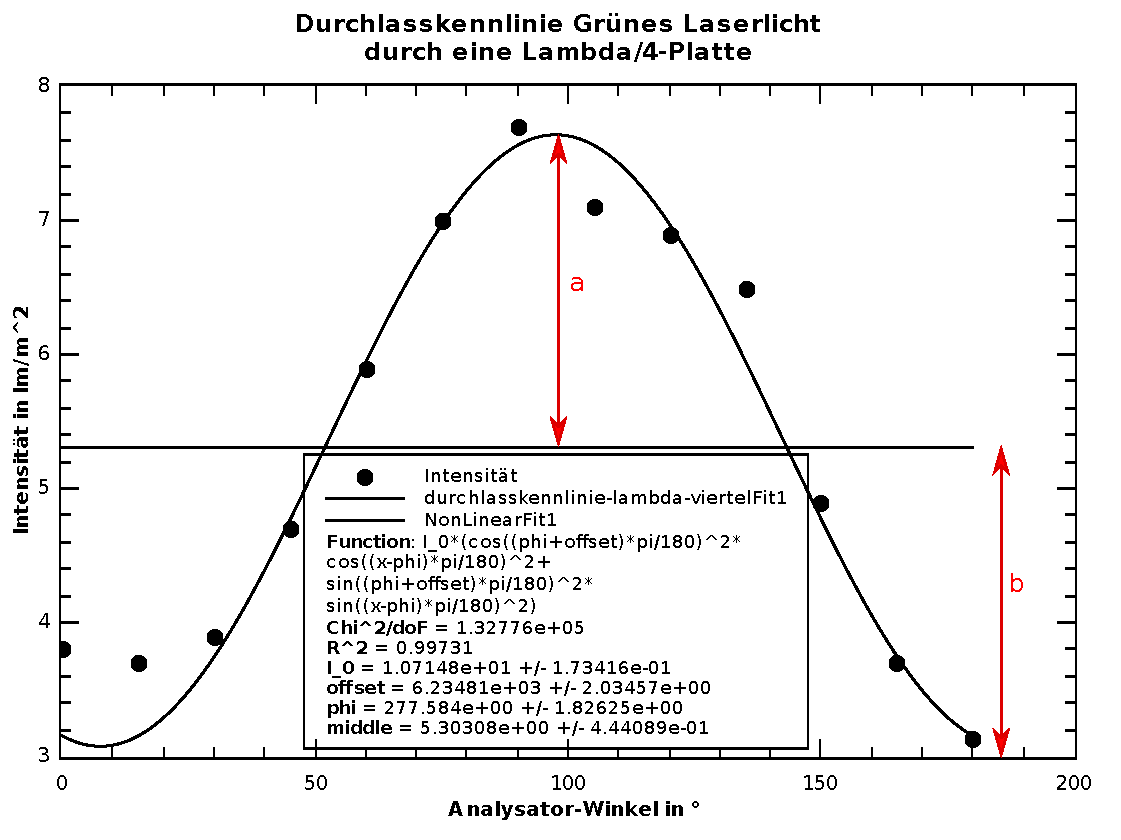
\includegraphics[width=.6\linewidth]{images/aufgabe-6.pdf}
    \caption{}
\end{figure}

